\documentclass[preprint,linenumbers, longauthor]{aastex631}
\usepackage{graphicx}
\begin{document}

\title{The New Age of Big Data In Astronomy: A Review of on the SKA \& LSST}
\author{Mathew Icho}
\affiliation{The University of Illinois at Urbana-Champaign}

\begin{abstract}
I'm making my abstract my to do list for now

\textbf{1: Make my citations for the website in my intro better}

\textbf{2: Finish adding more details about the SDSS camera}

\textbf{3: Make figure 1 look better. Cite Gunn correctly}
\end{abstract}

\tableofcontents

\section{Introduction}
%Start with kind of a summarized overview with the paper
%Then go to history of data being handled in Astronomy
%Then go talk about Moore's law%Then talk about main idea of this paper, say how its gonna be structured
The concept of data has long been a principal concern throughout the history of astronomy. Data allows scientists to discover natural laws in the universe, have control over events, and make reliable predictions. It has played a critical role in other time-sensitive fields such as medicine and engineering, where accurate data is essential for decision-making and design. Although the nature of data varies fundamentally across different fields, one trend has remained consistent: the continual evolution of data science. As explained in The Fourth Paradigm \citep{heyFourthParadigmDataIntensive2009}, this evolution can be characterized through four successive paradigms. In the following sections, I describe the progression of data acquisition across these paradigms and illustrate each using examples from astronomy. I will then explain how SKA and LSST fit into this trajectory and exemplify the emerging era of data-intensive discovery.
\subsection{The Paradigms of Data Science}
The first and most primitive paradigm, as described by Hey, is empirical evidence. 
Empirical evidence refers to data collected through traditional means, such as direct observation or experimentation of natural phenomena using sensory perception or basic instruments. 
The primary purpose of empirical evidence is to identify patterns that allow scientists to develop a fundamental understanding of the natural world. 
Throughout much acquisition human history, empirical evidence represented the most prominent method for extracting knowledge from nature. 
An example of the first paradigm in astronomy is the career of Tycho Brahe, a Danish astronomer. Throughout his career in the 16th century, Brahe primarily collected and cataloged data on the position of astronomical bodies using naked-eye observations. 
However, this method of data collection is associated with several limitations. Empirical evidence can be compromised by human error, the precision of the instruments, and, most importantly, the relatively slow pace of data acquisition compared to subsequent paradigms.

The second paradigm is analytical evidence. Analytical evidence represents the second most prominent mode of scientific inquiry in terms of longevity. 
The primary purpose of analytical evidence is to construct mathematical formulas and theoretical frameworks based on empirical data. 
Unlike the first paradigm, which merely demonstrates that phenomena occur, the second paradigm seeks to explain why they occur. 
An example of the second paradigm in astronomy is the work of Johannes Kepler, a student of Tycho Brahe, who used Brahe's empirical observations to derive the laws of planetary motion \citep{heyFourthParadigmDataIntensive2009}. 
By transforming raw observational data into mathematical laws, Kepler exemplified how analytical evidence advances scientific understanding beyond description to explanation.

The third paradigm is simulation evidence, a relatively recent development with respect to the first two. The purpose of simulation evidence is to model natural phenomena that are too complex to solve analytically by hand. 
Its central role is to enable interpolation and extrapolation of data using computational techniques grounded in known physical laws. 
In astronomy, an example is the use of N-body simulations to study the dynamical evolution of planetary systems and galaxies. 
By simulating the gravitational interactions between multiple bodies simultaneously, astronomers can decipher theoretical structures and determine long-term behaviors that would be analytically impossible to solve.

The fourth and most recent paradigm is data-intensive science. 
This paradigm is characterized by the unprecedented scale, velocity, and complexity of data acquisition, driven in part by exponential advances in computational power and detector technologies, often associated with Moore's law. 
Unlike earlier paradigms, which focused on observation, theory, or simulation, data-intensive science emphasizes the ability to manage, analyze, and interpret vast datasets that exceed the capacity of traditional methods. 
While this exponential growth in data has enabled transformative discoveries, it also introduces significant challenges related to storage, processing, and accessibility. 

\subsection{The Rise of Big Data in Astronomy}
Astronomy has become one of the most prominent trailblazers of this paradigm. Modern observatories now generate petabyte-scale data that need new strategies for data management and analysis. 
The fourth paradigm in turn reshapes the scientific process itself. Instead of discoveries being made from observation or theory, they are now being made from interpreting massive data sets. 
However, these advances also expose alarming issues, including bottlenecks in the data pipeline, the storage of aforementioned data, the increase in skill needed to handle the data, and concerns regarding open access to data. 
The field of astronomy is both a beneficiary and a victim of this data-intensive transition. 

The exponential growth of data acquisition can be attributed to Moore's law. Moore's law is an observation coined by Cofounder of Intel, Gordon E. Moore in his paper titled, "Cramming more components onto integrated circuits". 
In said paper, Moore explains that the number of components that make up an integrated circuit increase approximately at a rate of a factor of 2 per year.
Moore also stated that this growth is not sustainable more many reasons, the most relevant being the fact that techniques to handle such complex circuits lag behind in terms of development \cite{mooreCrammingMoreComponents2006}.

Moore's law can be seen in many data-intensive fields, such as astronomy.
When applied, it explains both the recent development of Big Data in astronomy, and accurately predicts the present issue that methods being used for analyzing said data is lagging behind, causing the mentioned issues.

This paper therefore seeks to review the rise of Big Data in Astronomy and the technical and scientific issues surrounding it by examining four case studies: MeerKAT, The Sloan Digital Sky Survey (SDSS), The Legacy Survey of Space and Time (LSST), and The Square Kilometre Array (SKA). 
These facilities collectively highlight the scope of contemporary astronomical data, the methods of its acquisition, their relative successes, the ongoing challenges, and the solutions currently in use. I plan on doing this by reviewing the approach that all four case studies have taken or plan to take to collect data.

\subsection{A Qualitative Analysis of Relevant Survey Data}
To demonstrate the rise of Big Data in Astronomy, we must first examine the components that make up the SDSS. The SDSS is vital to this paper, as it is one of the earliest large-scale optical surveys that signifies the start of the fourth paradigm. 
Because of its relative early involement in the Big Data stage of astronomy, and its use of collecting optical data, I plan to compare the SDSS to LSST. The SDSS
consists of three main telescopes.

The first of the three is "The Sloan Foundation 2.5m Telescope". 
The Sloan Foundational Telescope is stationed at the Apache Point Observatory in New Mexico, where it observes the sky in the northern hemisphere. 
The Sloan foundational telescope is able to observe a 3$^\circ$ field of view through the use of its two corrector lenses, that help with distortion. \cite{gunn25TelescopeSloan2006}

Another vital telescope used in the SDSS project is "The Irénée du Pont Telescope at Las Campanas Observatory" . The Irénée du Pont Telescope differs from the 2.5m Telescope as it is stationed in Chile, where it observes the southern hemisphere instead. 
Similar to the first mentioned telescope, the Irénée du Pont Telescope displays a 2.1$^\circ$ field of view with only one corrector lens. \cite{bowenOpticalDesign40in1973}

The third yet most vital telescope is the "NMSU 1-meter Telescope". The NMSU telescope is stationed in the Apache Point Observatory alongside the Sloan Foundational Telescope. 
The NMSU telescope serves a purpose the former two don't because "Obtaining spectra of these bright sources is a challenge for the Sloan 2.5 m telescope and not practical through drilling and observing specialized plugplates" \cite{majewskiApachePointObservatory2017}. 
In essense, by using optical fibers connected to a spectrograph, the NMSU telescope observes stars that are too bright for the other two to observe. 
The combination of these telescopes allow for both optical data to be collected through multiple surveys \cite{holtzmanNMSU1Telescope2010}

the SDSS is made up of multiple subsurveys. The eBoss, a continuation of BOSS, utilize spectrographs to observe light at a wavelength range of 3600-10,400~\AA \cite{dawsonSDSSIVEXTENDEDBARYON2016}.
An additional subsurvey is the APOGEE-2, a continuation of APOGEE. It uses spectrographs similar to eBOSS, but APOGEE-2 collectes near-infrared objects \cite{majewskiApachePointObservatory2017}. 
MaNGA is a subsurvey that collect integral field unit measurements of 10,000 nearby galaxies using spectrographs \cite{bundyOVERVIEWSDSSIVMaNGA2014}.
MARVELS is another subservey that makes up the SDSS, it was built specifically to obtain radial velocity measurements of stars with high-precision in hopes of finding exoplanets \cite{bundyOVERVIEWSDSSIVMaNGA2014a}.


The MeerKAT is another survey essential to demonstrate how Big Data has evolved in the field of Astronomy.
MeerKAT became fully operational in 2018 in the Northern Cape Province of South Africa. It serves as a precursor to the Square Kilometre Array (SKA), as both facilities focus on the collection of radio data \cite{jonasMeerKATRadioTelescope2018}.
MeerKAT comprises 64 antennas distributed over a radius of approximately 600 miles. These antennas operate across frequency bands ranging from 350 MHz to 3500 MHz \cite{goedhartMeerKATSpecifications2025}.

MeerKAT has conducted and continues to conduct ten major survey projects. For the sake of conciseness, this discussion will focus on five of these surveys.
One is the "Looking At the Distant Universe with the MeerKAT Array" (LADUMA) survey.
The objective of the LADUMA survey is to "use HI observations to study galaxy evolution over two thirds of the age of the universe" \cite{blythLADUMALookingDistant2018}. 
LADUMA has used "shorter observations with MeerKAT's “Phase 1” (0.9-1.75 GHz) receivers
would be followed by longer observations in an expanded “Phase 4” (0.58-2.5 GHz) band" \cite{blythLADUMALookingDistant2018}.
Although the LADUMA survey is still ongoing, a portion of the data has already been released and will be discussed in the Methods section.

the MeerKAT Absorbtion Line Survey (MALS) is a survey conducted using MeerKAT using by collecting data about HI and OH absorvers at $z < 0.4$ and $z < 0.7$, where z is the redshift of a galaxy. 
The reason for using the HI observation specifically is because it is a descriptive tracer of the cold neutral medium in a galaxy. 
The cold neutral medium give scientist details on what the physical conditions of the interstellar medium of said galaxy is. This, in turn, allows scientists to extrapolate data on the star formation in the galaxy \cite{guptaBlindOHAbsorption2021}.

Another survey, the "The Hunt for Dynamic and Explosive Radio Transients with MeerKAT" (ThunderKAT), aims to find, identify and understand high-energy astrophysical processes via their radio emission (often in concert with observations at other wavelengths)." 
In essence, ThunderKAT analyzes radio data to catalogue high-energy phenomena, including supernovae, microquasars, and similar events \cite{woudtThunderKATMeerKATLarge2018}.

Another notable survey under MeerKAT is the MeerKAT HI Observations of Nearby Galactic Objects: Observing Southern Emitters (MHONGOOSE). this survey aims to catalogue the properties of HI gas in "around 30 nearby star-forming spiral and dwarf galaxies to extremely low H i column densities". 
MHONGOOSE is remarkable by its notably higher sensitivity compared to previous surveys such as HALOGAS and THINGS. This sensitivity is crucial for investigating how low-column-density gas influences the cosmic web and galactic accretion processes \cite{deblokMHONGOOSEMeerKATNearby2024}.

The final survey considered here is the "MeerKAT International GHz Tiered Extragalactic Exploration" (MIGHTEE). MIGHTEE utilizes radio data spanning 900–1670 MHz, achieving a resolution of approximately 6 arcseconds.

Together, these five surveys, along with the remaining projects, emphasize the pivotal role of MeerKAT in the era of Big Data astronomy. They are at the forefront of scientific research and are producing data volumes on the order of petabytes.

Having examined MeerKAT, its only natural to examine its successor, the SKA. The SKA has built on technical and scientific achievements paved by MeerKAT.
The SKA covers an area of approximately 3,000 km with antennas, which collect area up to 106 m$^2$ of the sky. Because of its astonishing techniqical prowess and complexity, The SKA represents the start of a new frontier for Big Data astronomy.
One technology being used is aperture synthesis, which allows for the signals from antennas to be in phase, allowing to reduce noise. Another innovation is the use of large centimeter wavelength antennas, which allow for data to travel across distances at high speeds. This, in turn, allows for data to be analyzed and processed quicker and optimized, which will be discussed in further detail in the Methods section. \cite{dewdneySquareKilometreArray2009}.

Alongside the SKA is its optical counterpart, the LSST, which similarly represents a major advance in the evolution of Big Data in astronomy
The LSST is a successor to the SDSS, as both projects observe optical data. The LSST, however, has much more sophisticated goals. The LSST plans to address 4 key scientific issues: Investigating dark energy and dark matter, cataloguing the solar system, collecting data for sky surveys, and mapping the Milky way.
To do all this, the LSST uses a 3.2-gigapixel camera with a sampling of 9.6 deg$^2$ field of view. These cameras are equipped with highly resistant sensors reinforced with silicon \cite{ivezicLSSTScienceDrivers2019}. All these inventions alongside others allow for the LSST to acquire complex and immense data sets never seen before.

Truly, the SDSS, MeerKAT, SKA, and LSST are the pinnacle of human ingenuiety. They will allow for unprecedented data rates for complex astrophysical events and phenomena.
In the following Methods section, I describe how the data is collected, processed, analyzed, and stored. I then compare SDSS and MeerKAT to their respective successor in order to address the issue of inflation of Big Data in astronomy.


\section{Methods}

%Methods:
%○ Approach to collecting Data
%● Talk about how the LSST and SKA are collecting data
%○ The nature of their data, ie the scope, type, etc
%■ LSST is optical imaging
%■ SKA is radio interferometry
%○ How they’re storing/archiving the data.
%○ How they’re generally processing their data
%○ Transparency of their respective Data pipeline
%○ Real time processing techniques (NOTE: NOT THE SAME AS THE METHODS
%DATA PROCESSING, THIS ONE IS FOR REAL TIME PROCESSING)
    %■ Show new techniques being developed to combat issues such as
    %optimization and time important issues

\textbf{The new text starts here:}
\subsection{Approach to collecting Data}
%LSST FIRST??
The methods section in this paper will methodically analyze the approaches that each four survey has taken.
First we will analyze properties with the data, such as the nature of the data, the scope, type, etc.
We will then discuss how the surveys are storing and archiving the data.
After that, we will talk about how they're processing their data generally.
And lastly, we will talk about how they are using real time processing.
The reason for using these four surveys is to compare the significant growth in big data in the field of astronomy.
This growth is important to discuss about as later in my discussion section, I will talk about how this exessive growth is
causing a cascade of issues because we simply cannot keep up.


The first survey we will talk about is the SDSS. The SDSS contains a 2.5 m telescope, which is vital to the SDSS.
The telescope is insanely complex, but I plan to talk about 5 main innovations the 2.5 m telescope has brought. I plan to do this by first explaining what the innovations of the telescopes broadly, then in detail. Last, I will explain how it factors in with collecting data.
The 2.5 m telescope had a crucial job; it had to observe the sky through optical data with extreme accuracy throughout years.
In order to do this big job, the 2.5 m telescope had 5 important innovations. 

\textbf{THE SDSS SECTION IS NOT DONE YET, add more detail about the camera and other stuff in the Gunn paper section 2.3. Its a little complex.}

The first innovation is the SDSS camera. According to Gunn et al.'s 2006 paper, the camera is made up of "30 2048 x 2048 SITe/Tektronix Charge-Coupled Devices (CCDs) and 24 2048 x 400 CCDS" \cite{gunn25TelescopeSloan2006}. 
A CCD is one of the most important detectors when it comes to converting observations into data in observational astronomy.
A CCD works by absorbing photons. These photons generate electrons due to the photoelectric effect. These electrons are run through a voltage over periods of time, which detect the amount of electrons. Lastly, the number is stored into a digital image pixel \cite{lesserSummaryChargeCoupledDevices2015}.


The second innovation of the 2.5 m Telescope is the efficient two fiber-fed double spectrographs that are able to obtain imaging data from 3800-9200 \AA \space and angles ranging from 0-$90^\circ$ \cite{gunn25TelescopeSloan2006}. 
In Gunn's 2006 paper, he compiles the results of the performance of the spectrographs.
\begin{figure}[h!]
  \centering
  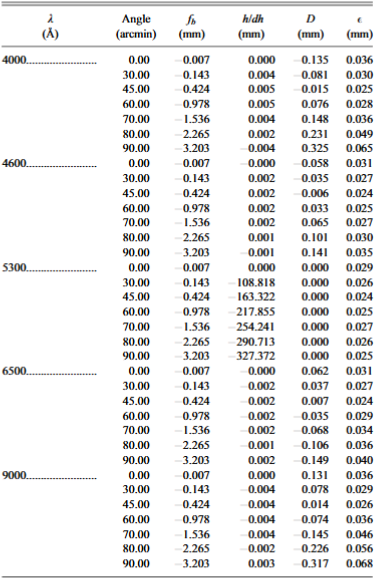
\includegraphics[width=0.4\textwidth]{gunn_table_5.png}
  \caption{Figure 5 of Gunn's 2006 Paper}
  \label{fig:SDSS_Table}
\end{figure}

In figure 5, $\lambda$ symbolizes the wavelength of light. Angle symbolizes the field angle. $f_b$ symbolzies the best-focus distance, which is the position that gives the best focus.
$h/dh$ symbolizes the lateral color. $D$ represents the longitutal differences from the best focus. Lastly, $\epsilon$ is the rms image diameter.
The second innovation of the 2.5 m Telescope is the efficient two fiber-fed double spectrographs that are able to obtain imaging data from 3800-9200 \AA \space and angles ranging from 0-$90^\circ$ \cite{gunn25TelescopeSloan2006}. 

The more important symbols to observe are the lateral color and longitutal differences. \textbf{maybe explain what these two things are? Do more research to figure out what a good number for these 2 are}. 
The closer to 0 these parameters are, the higher quality the resolution of an image is. According to Figure 5 of Gunn's Paper, throughout all wavelengths and angles besides 5300-6500, the lateral color and longitutal differeences are nearly 0.
All in all, the SDSS camera is extremely effective.

The third innovation of the 2.5 m telescope is a data acquisition system that accurately assesses data and stores it accordingly while using real-time processing to maintain quality \cite{gunn25TelescopeSloan2006}.






Next there is the LSST
\subsection{Real Time Processing}

\subsection{Transparency of their respective Data Pipeline}
\bibliography{references}

\end{document}

